\documentclass[10pt]{article}

\usepackage[margin=0.82in,top=0.78in,bottom=0.82in]{geometry}
\usepackage[T1]{fontenc}
\usepackage{lmodern}
\usepackage{microtype}
\usepackage{amsmath,amssymb}
\usepackage{booktabs}
\usepackage{graphicx}
\usepackage{xcolor}
\usepackage{titlesec}
\usepackage{caption}
\usepackage{enumitem}
\usepackage[colorlinks=true,linkcolor=accentblue,citecolor=accentblue,urlcolor=accentblue]{hyperref}

\definecolor{accentblue}{HTML}{1D4ED8}
\definecolor{navy}{HTML}{0F172A}
\definecolor{softbg}{HTML}{F1F5F9}
\definecolor{softborder}{HTML}{93C5FD}
\definecolor{warmbg}{HTML}{FFFBEB}
\definecolor{warmborder}{HTML}{FCD34D}
\definecolor{muted}{HTML}{475569}

\linespread{1.08}
\setlength{\parskip}{5pt}
\setlength{\parindent}{0pt}
\setlength{\textfloatsep}{12pt plus 2pt minus 2pt}
\setlength{\floatsep}{10pt plus 2pt minus 2pt}
\setlength{\intextsep}{10pt plus 2pt minus 2pt}
\setlength{\abovedisplayskip}{7pt}
\setlength{\belowdisplayskip}{7pt}

\titleformat{\section}{\large\sffamily\bfseries\color{navy}}{\thesection}{0.7em}{}
\titleformat{\subsection}{\normalsize\sffamily\bfseries\color{accentblue}}{\thesubsection}{0.6em}{}
\titlespacing*{\section}{0pt}{14pt plus 3pt minus 2pt}{5pt plus 1pt}
\titlespacing*{\subsection}{0pt}{10pt plus 2pt minus 1pt}{3pt plus 1pt}

\captionsetup{
  font=small,
  labelfont={bf,sf,color=navy},
  textfont={color=muted},
  skip=5pt
}

\setlist[itemize]{leftmargin=1.4em,itemsep=3pt,topsep=3pt}

% Clean callout box macro (zero exotic package dependencies)
\newcommand{\takeawaybox}[2]{%
  \vspace{4pt}
  \noindent\fcolorbox{softborder}{softbg}{%
    \begin{minipage}{\dimexpr\textwidth-2\fboxsep-2\fboxrule\relax}
      \vspace{3pt}
      {\sffamily\bfseries\small\color{accentblue} #1}\par\vspace{3pt}
      \small #2
      \vspace{3pt}
    \end{minipage}%
  }%
  \vspace{5pt}
}

\newcommand{\neff}{N_{\mathrm{eff}}}
\newcommand{\nvis}{N_{\mathrm{vis}}}
\newcommand{\R}{\mathbb{R}}

\begin{document}

% --- Clean Title Block ---
\begin{center}
  {\LARGE\sffamily\bfseries\color{navy} Improving Out-of-Distribution Generalization with\\[3pt]
  Bias-Aware Softmax Scaling and Barrier-FoX}\\[6pt]
  {\large\sffamily\color{muted} From 200-Digit Arithmetic Circuits to Sub-40s 8$\times$H100 LLM Training}\\[10pt]
  {\normalsize Felipe Sens Bonetto \quad $\cdot$ \quad \texttt{felipesensbonetto@gmail.com}}
\end{center}

\vspace{4pt}

\begin{abstract}
\noindent
Self-attention fails in two simple, fixable ways when sequence lengths change or hard boundaries appear.
First, \textbf{attention does not know how many keys it can actually see.} When queries and keys are normalized, dot products stay bounded while more tokens dilute softmax weights. Prior fixes (Scalable Softmax) sharpen every query using $\log(\text{position}+1)$, assuming every earlier token is visible---which breaks as soon as sliding windows, packed document boundaries, or decay masks hide most of the prefix.
Second, \textbf{fixed distance decay cannot act like a switch.} Static slopes decay smoothly with distance, so a head cannot transmit an unbroken carry chain ($a_k+b_k=9$) with zero loss while blocking everything past the first carry-breaker ($a_k+b_k\neq 9$).

We fix both with two minimal, strictly causal mechanisms:
\textbf{(1)~Bias-Aware SSMax} counts only the effective keys that \emph{survive} the attention mask or bias, centers the scaling curve around a neutral length so short contexts soften while long windows sharpen, and starts at exact identity ($\tau=1$). On modern sliding-window language models it simplifies to a closed-form $O(T)$ count with zero attention-kernel changes and only $+1$ scalar per head.
\textbf{(2)~Place-Ordered Barrier-FoX} lets each token raise a learned non-negative wall ($g \ge 0$) accumulated along the right causal axis (digit place order for arithmetic; token order with a dead-zone $\operatorname{ReLU}$ gate for general sequences).

Opening the learned models reveals crisp, human-readable circuits in both small algorithmic Transformers and a $124\text{M}$ LLM:
(i)~On addition trained only on $1,2,3,5$-digit numbers, all $9/9$ seeds spontaneously discover hardware \emph{carry-lookahead walls} (transparent on $a_k+b_k=9$, opaque walls on $<9$ and $>9$), lifting $25$-digit ($5\times$) accuracy by $+59\text{pp}$, extrapolating up to $81.2\%$ at $200$ digits ($40\times$), and collapsing from $97.7\% \to 0.0\%$ when only those walls are zeroed.
(ii)~On multi-step symbolic algebra with zero digit formulas, general causal versions yield $3.7\times$ exact match on $2\times$ longer traces ($+17.2\text{pp}$ token accuracy, $p=0.0033$).
(iii)~On the $124\text{M}$ \texttt{modded-nanogpt} speedrun, Bias-Aware SSMax adds just $+42$ scalars fused into QK-RMSNorm+RoPE with zero extra HBM passes ($+72\text{ ms}$, $+0\text{ MiB}$ VRAM): $250/252$ heads learn positive slopes with long-window layers learning $2.5\times$ steeper curves, run-to-run loss variance drops $3.5\text{--}4.9\times$, and an official interleaved $10\text{ vs.\ }10$ certification on $8\times\text{H100 SXM5}$ cuts training time by $-0.477\text{ s}$ ($40.45\text{ s} \to \mathbf{39.98\text{ s}}$, $p=7.6\times 10^{-12}$) while clearing the $3.28$ validation gate on $10/10$ runs ($p=1.26\times 10^{-6}$), whereas cutting steps without SSMax fails the gate ($p=0.496$).
\end{abstract}

% =============================================================================
\section{Two Simple Blind Spots in Self-Attention}
\label{sec:intro}

Modern Transformers normalize their queries and keys before taking dot products (QK-RMSNorm). That keeps training stable, but because every query and key sits on a fixed-radius sphere, the largest possible logit margin between the right token and a distractor cannot grow when the context gets longer. As more tokens enter the softmax denominator, attention weights wash out~\cite{chiang2022,velickovic2025}.

Scalable-Softmax (SSMax)~\cite{nakanishi2025} proposed a clean fix: multiply each query by $s_h \log(t+1)$ so later tokens get sharper attention. But real Transformers almost never let every token attend uniformly to all $t+1$ earlier tokens. Language models pack many unrelated documents into one long batch separated by \texttt{<|endoftext|>} resets and cap most layers with a short sliding window $W_\ell$. Algorithmic models use local biases and learned decay gates. In all of these settings, $\log(t+1)$ \emph{lies} about how many tokens are actually competing (Figure~\ref{fig:intuition}a): on the very first token of a new packed document, $\log(t+1)$ thinks over a thousand tokens are visible when only \emph{one} token is.

A second blind spot shows up whenever a model must route information over an arbitrary number of steps until a stopping condition occurs---such as propagating a carry across fifty consecutive $9$-columns in addition, or ignoring finished scratchpad lines in multi-step algebra. Fixed distance penalties like ALiBi~\cite{press2022} decay at one constant rate everywhere, so they cannot simultaneously pass a carry-propagating column ($a_k+b_k=9$) with \emph{zero} decay and block everything past a carry-breaking column ($a_k+b_k\neq 9$). Learned forget gates like FoX~\cite{lin2025} can act like walls, but accumulating walls along raw token order runs \emph{backwards} on left-to-right addition (Figure~\ref{fig:intuition}c).

\begin{figure}[t]
  \centering
  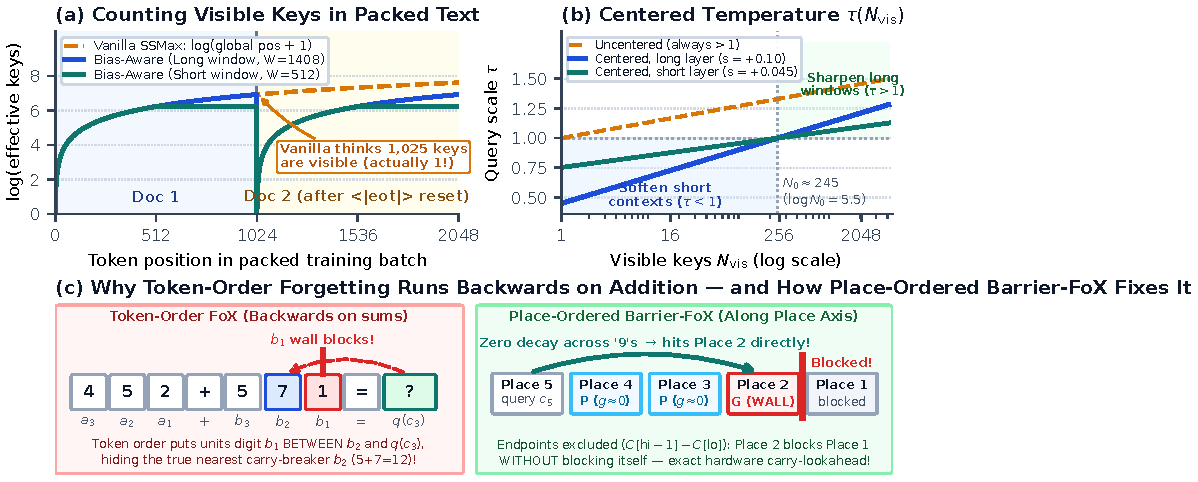
\includegraphics[width=\textwidth]{fig1_intuition.pdf}
  \caption{\textbf{Plain-English picture of both mechanisms.}
  \textbf{(a)}~In a packed batch with document resets and sliding windows, Vanilla SSMax's $\log(\text{global pos}+1)$ over-counts keys right after every \texttt{<|eot|>} reset and beyond window $W_\ell$; Bias-Aware SSMax counts only the $N_{\mathrm{vis}}$ keys that survive the mask.
  \textbf{(b)}~Centering $\log N_{\mathrm{vis}}$ around $\log N_0 = 5.5$ ($N_0 \approx 245$) lets one positive slope $s_h$ gently \emph{soften} short contexts ($\tau < 1$) while \emph{sharpening} long windows ($\tau > 1$).
  \textbf{(c)}~On left-to-right addition, token-order forgetting places irrelevant lower digits ($b_1$) between the answer query and the nearest carry-breaker ($b_2$); Place-Ordered Barrier-FoX accumulates walls along digit places and excludes endpoints so a wall blocks everything behind it without blocking itself.}
  \label{fig:intuition}
\end{figure}

\takeawaybox{Summary of Contributions \& Headline Results}{
\begin{itemize}
  \item \textbf{Bias-Aware SSMax (\S\ref{sec:bssmax}):} Measures the exact number of keys surviving masks or additive biases, centers the temperature around a neutral length, and starts at exact identity ($\tau=1$). Beats naive Vanilla SSMax in \emph{every} domain we test---from $100$-digit addition ($26.0\%$ vs.\ $6.8\%$) to $33.5\text{M}$ FineWeb ($p=0.003$) to $124\text{M}$ \texttt{modded-nanogpt} ($-4.2\text{ mnat}$).
  \item \textbf{Place-Ordered Barrier-FoX \& Dead-Zone ReLU (\S\ref{sec:bfox}):} Fixes FoX's token-order inversion on arithmetic, yields $+59\text{pp}$ exact match at $5\times$ training length (up to $81.2\%$ at $40\times$), and spontaneously invents exact carry-lookahead walls across $9/9$ seeds (\S\ref{sec:add}). Replacing $\operatorname{softplus}$ with $\operatorname{ReLU}$ eliminates residual carry leakage ($42.2\% \to 71.9\%$ on $40$-digit pure-$9$ chains).
  \item \textbf{Sub-40s Certified $8\times\text{H100}$ LLM Training (\S\ref{sec:llm}):} Fusing Bias-Aware SSMax ($+42$ scalars) into \texttt{modded-nanogpt}'s QK-RMSNorm+RoPE Triton kernel adds $+72\text{ ms}$ ($+0.17\%$) and $+0\text{ MiB}$ VRAM, cuts run-to-run loss std by $3.5\text{--}4.9\times$, and reduces $8\times\text{H100 SXM5}$ training time from $40.45\text{ s} \to \mathbf{39.98\text{ s}}$ ($-0.477\text{ s}$, $10/10$ runs below $3.2784$, $p=1.26\times 10^{-6}$).
\end{itemize}}

% =============================================================================
\section{How Both Mechanisms Work}
\label{sec:method}

\subsection{Bias-Aware Scalable Softmax (Bias-Aware SSMax)}
\label{sec:bssmax}

Suppose query $i$ in head $h$ receives causal additive attention bias $B_{i,j,h} \in \R \cup \{-\infty\}$ (where masked or future keys have $B_{i,j,h} = -\infty$). How many keys effectively survive $B$ before content dot products are even added? Look at the partition function of $B$ shifted by its maximum:
\begin{equation}
  \log \neff(i, h) \;=\; \operatorname{logsumexp}_{j \le i}(B_{i,j,h}) - \max_{j \le i}(B_{i,j,h}) \;\in\; \big[0,\; \log(i+1)\big].
  \label{eq:neff}
\end{equation}
Two sanity checks show why Eq.~\eqref{eq:neff} is the exact right quantity:
\begin{itemize}
  \item If all $k$ visible keys have equal bias $0$ (and all others are $-\infty$), then $\operatorname{logsumexp} = \log k$ and $\max = 0$, so $\neff = k$ exactly.
  \item If a local bias or barrier suppresses every key except $O(1)$ neighbors, then $\neff = O(1)$ even in a $1{,}000$-token sequence---so local heads never get artificially over-sharpened. Adding any constant to row $i$ shifts both terms identically and cancels out.
\end{itemize}
We detach $\log \neff$ (so it acts purely as a geometric ruler, not a backdoor gradient into $B$) and multiply queries right before attention by a clamped linear temperature with one learned scalar $s_h$ per head:
\begin{equation}
  \tau_{i,h} \;=\; \max\!\Big(0.25,\; 1 + s_h\big(\log \neff(i, h) - c\big)\Big), \qquad \tilde{q}_{i,h} \;=\; \tau_{i,h}\, q_{i,h}.
  \label{eq:tau}
\end{equation}
We initialize $s_h = 0$ with zero weight decay, so at step $0$ the model starts at exact identity ($\tau = 1$) with no optimization shock.

\textbf{Why the center $c$ matters (and why LLM training needs zero $O(T^2)$ work).}
In standard LLM stacks like \texttt{modded-nanogpt}~\cite{jordan2024}, attention uses hard causal masks, hard \texttt{<|endoftext|>} document boundaries, and hard per-layer sliding windows of width $W_\ell$. There is no soft bias matrix to sum over: Eq.~\eqref{eq:neff} collapses analytically into an $O(T)$ formula per token $t$:
\begin{equation}
  \nvis(t, \ell) \;=\; \min\!\big(\mathrm{pos\_in\_doc}(t) + 1,\; W_\ell\big),
  \label{eq:nvis}
\end{equation}
(and $\min(2\,\mathrm{pos\_in\_doc}(t),\, W_\ell)$ on paired-head layers whose interleaved stream doubles the local key count inside window $W_\ell$).

In our $124\text{M}$ LLM ablations (\S\ref{sec:llm}), centering at $c = 5.5$ ($N_0 = e^{5.5} \approx 245$ tokens, near the midpoint of the training windows) proved decisive. Without centering ($c = 0$), a single positive slope can only \emph{increase} temperature ($\tau \ge 1$ everywhere). With centering ($c = 5.5$, Figure~\ref{fig:intuition}b), the \emph{same} single scalar $s_h > 0$ softens the very start of each document ($\tau < 1$, preventing early-token over-confidence) while sharpening queries once hundreds or thousands of tokens fill the window ($\tau > 1$).

\subsection{Place-Ordered Barrier-FoX and Dead-Zone ReLU Gates}
\label{sec:bfox}

Forgetting Attention (FoX)~\cite{lin2025} gives each token a learned non-negative wall height $g_{k,h} \ge 0$ and subtracts the sum of walls strictly between key $j$ and query $i$ from the attention logit. On general text or multi-step reasoning (\S\ref{sec:expr}--\S\ref{sec:fineweb}), accumulating walls along token order works naturally (\textbf{Token-FoX}): a newline or topic shift can emit a high wall so later tokens forget obsolete scratchpad lines.

On left-to-right (MSB-first) addition, however, token order is inverted relative to carry flow (Figure~\ref{fig:intuition}c). To predict answer digit $c_p$, the model must scan rightwards to lower places ($p-1, p-2, \dots$) to find the nearest column $q < p$ where $a_q + b_q \neq 9$. In token order, irrelevant lower-order digits $b_1, \dots, b_{q-1}$ sit \emph{between} $b_q$ and the answer token---so any wall at $b_1$ blinds the query to $b_q$.

\textbf{Place-Ordered Barrier-FoX} fixes this while remaining $100\%$ causal in token order. Each token $k$ computes a non-negative barrier $g_{k,h} = \phi(W_{g,h}^\top \operatorname{RMSNorm}(x_k) + b_{g,h}) \ge 0$ ($\phi \in \{\operatorname{softplus}, \operatorname{ReLU}\}$; zero on non-digit tokens). At query step $i$, we sum barriers emitted so far ($k \le i$) into each digit place $p \in \{1,\dots,P\}$, take a prefix sum along places, and subtract only the walls \emph{strictly between} $\mathrm{lo}=\min(p_i,p_j)$ and $\mathrm{hi}=\max(p_i,p_j)$:
\begin{equation}
  S_{i,p,h} = \sum_{\substack{k \le i \\ \mathrm{pid}_k = p}} g_{k,h}, \qquad
  C_{i,p,h} = \sum_{r=1}^{p} S_{i,r,h}, \qquad
  D_{i,j,h} = \mathbf{1}_{[\mathrm{hi}-\mathrm{lo} \ge 2]}\big(C_{i,\mathrm{hi}-1,h} - C_{i,\mathrm{lo},h}\big).
  \label{eq:bfox}
\end{equation}
Subtracting $D_{i,j,h}$ from the attention bias before Eq.~\eqref{eq:neff} satisfies four exact invariants (all unit-tested):
(1)~\emph{strict causality} (only $k \le i$ enters $S_{i,\cdot,h}$),
(2)~\emph{exact place-shift invariance} (adding any constant $+c$ to all place IDs leaves logits unchanged),
(3)~\emph{monotonicity / zero periodic aliasing} ($g_{k,h} \ge 0$), and
(4)~\emph{self-visibility} (excluding both endpoints means a carry-breaker at place $q$ blocks every column $r < q$ \emph{without blocking itself}).
Because $\operatorname{softplus}(z)$ is strictly positive everywhere, even a tiny residual $g \approx 0.05$ leaks $40 \times 0.05 = 2.0$ logits across a $40$-digit chain of $9$s; switching to a \textbf{dead-zone $\operatorname{ReLU}$ gate} lets transparent tokens output \emph{literal $0.000$}.

% =============================================================================
\section{Opening the Black Box: Carry-Lookahead Circuits \& \texorpdfstring{40$\times$}{40x} Addition Extrapolation}
\label{sec:add}

\textbf{Setup.} We test length extrapolation on a strict ``skip-4'' addition protocol~\cite{mcleish2024}: models train for $5{,}000$ AdamW steps exclusively on $1, 2, 3,$ and $5$-digit sums (\texttt{\textbackslash n a + b = c \textbackslash n}; $4$-digit sums completely held out) and are evaluated on fixed unseen sums from $6$ digits up to $200$ digits ($40\times$ longer than training). Our alias-free backbone (\texttt{NeoGPT v2}) is a $4$-layer, $4$-head NoPE Transformer with QK-RMSNorm, SwiGLU~\cite{shazeer2020}, clipped local bias, and monotonic log-place distance bias, tested at both $112\text{k}$ ($d=48$) and $1.27\text{M}$ ($d=160$) parameters ($n=3$ seeds per arm), plus a Place-RoPE baseline (\texttt{v1.1}, random place scaling $s \sim \mathcal{U}[1,2]$).

\begin{figure}[t]
  \centering
  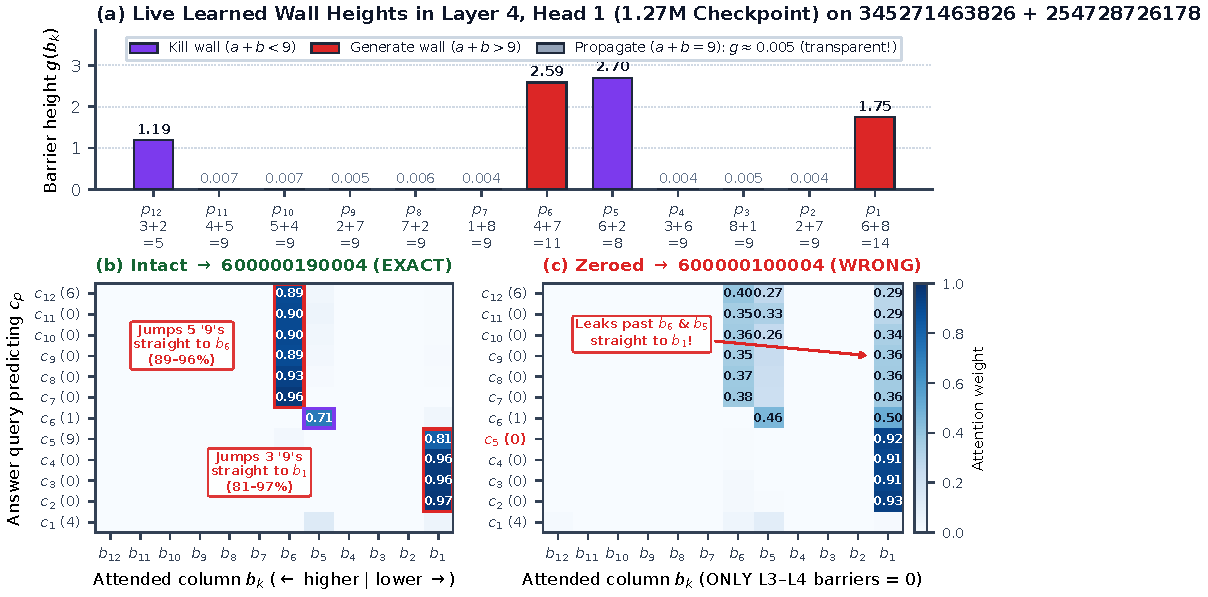
\includegraphics[width=\textwidth]{fig2_mech_carry.pdf}
  \caption{\textbf{Opening the black box on live trained weights ($1.27\text{M}$ seed 1, Layer 4 Head 1).}
  We feed a $12$-digit sum containing a $5$-digit carry chain ($p_{11}\text{--}p_7$) and a $3$-digit carry chain ($p_4\text{--}p_2$): $345271463826 + 254728726178 = 600000190004$.
  \textbf{(a)}~Without any supervision on carry classes, the learned barrier gate emits sharp walls ($1.19\text{--}2.70$) on every \emph{Kill} ($a+b<9$) and \emph{Generate} ($a+b>9$) column, and drops to $0.004\text{--}0.007$ on every \emph{Propagate} ($a+b=9$) column.
  \textbf{(b)}~Intact post-barrier attention forms an exact hardware carry-lookahead staircase: queries $c_{12}\text{--}c_7$ jump over five $9$-columns straight onto $b_6$ ($89\text{--}96\%$ weight), $c_6$ stops at Kill column $b_5$ ($71\%$), and $c_5\text{--}c_2$ jump over three $9$-columns onto $b_1$ ($81\text{--}97\%$), outputting the exact answer.
  \textbf{(c)}~Zeroing \emph{only} Layer 3--4 barrier weights at inference leaves every other weight untouched, yet attention immediately leaks past $b_6$ and $b_5$ straight to $b_1$ and corrupts the answer ($c_5: 9 \to 0$).}
  \label{fig:mech_carry}
\end{figure}

\subsection{Mechanistic Interpretability: The Model Invents Hardware Carry-Lookahead}

In digital circuit design, fast adders classify every digit column $k$ into three states:
\emph{Kill} ($a_k+b_k < 9$, stops incoming carry),
\emph{Propagate} ($a_k+b_k = 9$, passes incoming carry untouched), and
\emph{Generate} ($a_k+b_k > 9$, emits a new carry and stops older ones).

Remarkably, across \textbf{9 out of 9 independently trained $\operatorname{softplus}$ Barrier-FoX seeds} ($6$ at $112\text{k}$ and $3$ at $1.27\text{M}$), gradient descent spontaneously discovers this exact algebra inside Layers 3--4. Figure~\ref{fig:mech_carry}a shows the live barrier heights emitted by Layer 4, Head 1 of our $1.27\text{M}$ seed 1 checkpoint on a concrete $12$-digit sum: every Kill and Generate column raises a $1.19\text{--}2.70$ wall, while all eight Propagate columns sit flat at $0.004\text{--}0.007$ (up to $675\times$ smaller!).

Figure~\ref{fig:mech_carry}b shows what that barrier profile does to attention: every answer query $c_p$ scans right across any number of transparent $9$-columns and locks with $71\text{--}97\%$ attention weight onto the \emph{exact} nearest carry-breaker column, stopping dead at the wall behind it. To prove these walls are causally responsible---and not mere correlated features---Figure~\ref{fig:mech_carry}c zeroes \emph{only} the Layer 3--4 barrier projections at inference while leaving every other matrix intact ($W_Q, W_K, W_V, W_O$, MLPs, embeddings, biases). Instantly, attention bleeds past $b_6$ and $b_5$ down to $b_1$ and the model outputs the wrong digit. Across four tested checkpoints, zeroing only Layer 3--4 barrier gates collapses $25$-digit accuracy by \textbf{53--98 percentage points} (Figure~\ref{fig:add_results}b), including a complete $97.7\% \to 0.0\%$ collapse on $1.27\text{M}$ seed 2.

\begin{figure}[t]
  \centering
  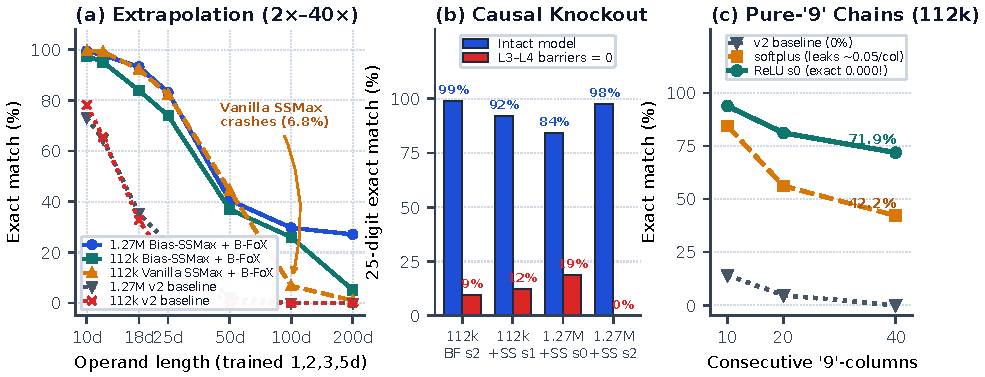
\includegraphics[width=\textwidth]{fig3_addition_results.pdf}
  \caption{\textbf{Addition extrapolation, causal knockout, and dead-zone ReLU verification.}
  \textbf{(a)}~Exact match from $10\text{d}$ ($2\times$) to $200\text{d}$ ($40\times$ training length, $n=3$): Bias-Aware SSMax + Barrier-FoX sustains extrapolation to $100\text{d--}200\text{d}$, whereas Vanilla SSMax over-sharpens barrier-truncated heads and crashes from $44.5\%$ ($50\text{d}$) to $6.8\%$ ($100\text{d}$).
  \textbf{(b)}~Zeroing \emph{only} Layer 3--4 barrier gates at inference destroys $25$-digit accuracy across every tested checkpoint (up to $97.7\% \to 0.0\%$).
  \textbf{(c)}~On adversarial contiguous pure-$9$ carry chains ($N=64$, $112\text{k}$), strictly positive $\operatorname{softplus}$ leaks $\sim 0.05$ logits per column and caps at $42.2\%$ on $40$-digit chains; dead-zone $\operatorname{ReLU}$ drives Propagate columns to literal $0.000$ and jumps to $71.9\%$.}
  \label{fig:add_results}
\end{figure}

\begin{table}[t]
  \centering
  \caption{Skip-4 addition exact match (\%, mean$\pm$std, $n=3$ seeds) trained only on $1,2,3,5$-digit operands. Bias-Aware SSMax and Barrier-FoX stack synergistically at both $112\text{k}$ and $1.27\text{M}$ scale; Vanilla SSMax crashes past $50\text{d}$.}
  \label{tab:add}
  \footnotesize
  \renewcommand{\arraystretch}{1.14}
  \setlength{\tabcolsep}{2.2pt}
  \begin{tabular}{@{}lrccccccc@{}}
    \toprule
    Model ($n=3$ seeds) & Params & 6d & 10d & 18d & \textbf{25d (5$\times$)} & \textbf{50d (10$\times$)} & \textbf{100d (20$\times$)} & \textbf{200d (40$\times$)} \\
    \midrule
    $112\text{k}$ \texttt{v1.1} (Place-RoPE) & 112k & 97.6$\pm$2.2 & 20.8$\pm$12.1 & 0.0 & 0.0 & 0.0 & 0.0 & 0.0 \\
    \midrule
    $112\text{k}$ \texttt{v2} base (NoPE+log) & 112k & 99.5$\pm$0.6 & 78.2$\pm$10.1 & 32.8$\pm$16.6 & 15.3$\pm$14.4 & 0.0$\pm$0.0 & 0.0$\pm$0.0 & 0.0$\pm$0.0 \\
    \quad $+$ Bias-SSMax & 112k & 99.8$\pm$0.2 & 85.1$\pm$14.2 & 44.0$\pm$35.7 & 28.4$\pm$35.8 & 3.4$\pm$5.9 & 0.0$\pm$0.0 & 0.0$\pm$0.0 \\
    \quad $+$ Barrier-FoX & 113k & 97.6$\pm$4.1 & 91.3$\pm$9.5 & 66.4$\pm$32.8 & 61.2$\pm$39.1 & 31.5$\pm$26.7 & 13.0$\pm$18.7 & 5.2$\pm$9.0 \\
    \quad $+$ Vanilla SSMax + B-FoX & 113k & 100.0$\pm$0.0 & \textbf{99.5$\pm$0.9} & \textbf{92.2$\pm$12.2} & \textbf{82.3$\pm$28.0} & \textbf{44.5$\pm$39.4} & 6.8$\pm$9.2 & 1.0$\pm$1.8 \\
    \quad $+$ Bias-SSMax + B-FoX (ReLU) & 113k & 99.9$\pm$0.2 & 88.5$\pm$17.3 & 70.8$\pm$24.2 & 56.8$\pm$18.6 & 28.1$\pm$15.8 & 5.7$\pm$5.0 & 1.0$\pm$1.8 \\
    \quad \textbf{$+$ Bias-SSMax $+$ B-FoX} & \textbf{113k} & \textbf{100.0$\pm$0.0} & 97.5$\pm$3.8 & 83.9$\pm$16.6 & 74.0$\pm$19.2 & 37.0$\pm$33.6 & \textbf{26.0$\pm$23.4} & \textbf{5.2$\pm$9.0} \\
    \midrule
    $1.27\text{M}$ \texttt{v2} base (NoPE+log) & 1.27M & 99.2$\pm$0.6 & 73.1$\pm$13.5 & 35.4$\pm$21.1 & 23.4$\pm$18.9 & 2.3$\pm$4.0 & 0.0$\pm$0.0 & 0.0$\pm$0.0 \\
    \quad \textbf{$+$ Bias-SSMax $+$ B-FoX} & \textbf{1.28M} & \textbf{100.0$\pm$0.0} & \textbf{99.4$\pm$0.9} & \textbf{93.2$\pm$4.7} & \textbf{83.1$\pm$15.3} & \textbf{40.6$\pm$21.5} & \textbf{29.7$\pm$28.7} & \textbf{27.1$\pm$46.9}$^\dagger$ \\
    \bottomrule
  \end{tabular}
  \vspace{2pt}
  \parbox{\textwidth}{\footnotesize\color{muted} $^\dagger$Per-seed $1.27\text{M}$ champion ($25\text{d}/50\text{d}/100\text{d}/200\text{d}$): s0~$84.4/61.7/62.5/\mathbf{81.2\%}$ (26/32 exact at $200\text{d}$); s1~$67.2/18.8/9.4/0.0\%$; s2~$\mathbf{97.7}/41.4/17.2/0.0\%$.}
\end{table}

\subsection{Extrapolation, Negative Controls, and Fixing Softplus Leakage}

Table~\ref{tab:add} and Figure~\ref{fig:add_results}a summarize the full factorial sweep:
\begin{itemize}
  \item \textbf{Synergistic extrapolation:} Combining Bias-Aware SSMax ($+16$ scalars) and Barrier-FoX ($+784$ params at $112\text{k}$) lifts $25$-digit ($5\times$) exact match from $15.3\% \to \mathbf{74.0\%}$ at $112\text{k}$ ($+58.6\text{pp}$, two-sided Welch $p=0.0157$) and from $23.4\% \to \mathbf{83.1\%}$ at $1.27\text{M}$ ($+59.7\text{pp}$, $p=0.0145$). On $1.27\text{M}$ seed 0---which pushed its Layer 4 Head 3 Propagate barrier all the way down to $0.00$---accuracy reaches $\mathbf{81.2\%}$ at $200$ digits ($40\times$ training length).
  \item \textbf{Why Bias-Aware beats Vanilla SSMax:} On \texttt{v2+B-FoX}, Vanilla SSMax scales by raw $\log(i+1)$ even after barriers have trimmed each head to a handful of unblocked keys. That extra sharpening helps at $10\text{d--}50\text{d}$ but over-sharpens and collapses past $50\text{d}$, dropping to $6.8\%$ at $100\text{d}$ ($3.8\times$ worse than Bias-Aware's $26.0\%$). On Place-RoPE \texttt{v1.1}, Bias-Aware beats Vanilla at every OOD length ($8\text{d}$ EMA $68.6\%$ vs.\ $60.3\%$) while cutting seed std in half ($\pm 14.5$ vs.\ $\pm 32.3$). Two negative controls that \emph{soften} attention on \texttt{v1.1} (Partition-Function Stretch and Attention Score Decay $10^{-4}$) drop $10\text{d}$ EMA from $23.0\% \to 8.5\%$ and $7.0\%$, matching $10\text{d}$ attention sharpness with exact rank correlation ($\rho = 1.00$).
  \item \textbf{Testing the softplus-leakage prediction:} On synthetic sums containing $40$ consecutive $9$-columns (Figure~\ref{fig:add_results}c), strictly positive $\operatorname{softplus}$ leaks $40 \times 0.05 \approx 2.0$ logits and plateaus at $42.2\%$. Swapping in dead-zone $\operatorname{ReLU}$ drives four carry heads in seed 0 to \textbf{literal $0.000$ on $100\%$ of Propagate columns} and jumps $40$-digit chain accuracy to $\mathbf{71.9\%}$---confirming the diagnosis, while honestly revealing a dead-ReLU seed-variance trade-off on random sums ($56.8\%$ vs.\ $74.0\%$ at $25\text{d}$).
\end{itemize}

% =============================================================================
\section{Generalization Without Digit Formulas: Multi-Step Symbolic Algebra}
\label{sec:expr}

Place-Ordered Barrier-FoX uses digit place coordinates specific to arithmetic. Does our approach still win when there are \textbf{zero digit coordinates and zero task-specific length formulas}? We test canonical step-by-step rewriting of nested exact-rational expressions with $+, -, \times, \div$, and parentheses (evaluated with Python \texttt{Fraction}, e.g., \texttt{(17*22)/(18+321+4122451)-123+34/12} reduced over $15$ exact lines). We compare two matched $4\text{L}\,4\text{H}\,d=96$ models ($n=3$ seeds, exact KV-cached greedy rollout): \textbf{\texttt{NeoExprGPT}} ($447\text{k}$: NoPE + clipped local + ALiBi-log + strictly causal parenthesis-depth relative bias + general token-order \textbf{Token-FoX} + \textbf{Bias-Aware SSMax}) against a standard \textbf{\texttt{RoPE GPT}} baseline ($445\text{k}$).

\begin{table}[ht]
  \centering
  \caption{Multi-step exact-rational expression rewriting (EMA final \%, $n=3$ seeds). \textbf{(a)}~At full $18\text{k}$ convergence ($\sim 90\%$ \texttt{in\_dist}), \texttt{NeoExprGPT} beats \texttt{RoPE GPT} on every OOD split ($3/3$ seeds beat every RoPE seed on \texttt{ood\_steps} and \texttt{ood\_depth}). \textbf{(b)}~Component ablations at $6\text{k}$ confirm every piece is non-redundant.}
  \label{tab:expr}
  \footnotesize
  \renewcommand{\arraystretch}{1.14}
  \setlength{\tabcolsep}{3.5pt}
  \begin{tabular}{@{}lcccc@{}}
    \toprule
    Model ($n=3$ seeds) & \texttt{in\_dist} (1--3 ops) & \textbf{\texttt{ood\_steps}} (5--7 ops) & \textbf{\texttt{ood\_depth}} (3--4) & \texttt{ood\_scale} (4--5d) \\
    \midrule
    \multicolumn{5}{@{}l}{\textit{\textbf{(a) Full Convergence ($18\text{k}$ steps — final exact / full trace / token \%)}}} \\
    \texttt{RoPE GPT} ($445\text{k}$) & 87.5 / 82.6 / 99.2 & 4.2 / 4.2 / 79.2 & 28.5 / 25.7 / 91.2 & 10.4 / 10.4 / 86.9 \\
    \textbf{\texttt{NeoExprGPT}} ($447\text{k}$) & \textbf{89.6} / \textbf{84.0} / \textbf{99.3} & \textbf{15.3} / \textbf{13.9} / \textbf{96.4} & \textbf{43.1} / \textbf{43.1} / \textbf{98.3} & \textbf{15.3} / \textbf{14.6} / \textbf{88.7} \\
    $\Delta$ (paired $p$ on tok) & $+2.1$ / $+0.1\text{pp}$ & \textbf{$3.7\times$} / \textbf{$+17.2\text{pp}$ (.0033)} & \textbf{$+14.6\text{pp}$} / \textbf{$+7.1\text{pp}$ (.0038)} & $+4.9$ / $+1.7\text{pp}$ \\
    \midrule
    \multicolumn{5}{@{}l}{\textit{\textbf{(b) Component Ablations ($6\text{k}$ steps — final exact / token \%)}}} \\
    \textbf{\texttt{NeoExprGPT} Full} ($447\text{k}$) & \textbf{57.6$\pm$9.8} / \textbf{97.6} & \textbf{2.1$\pm$2.1} / \textbf{94.6} & \textbf{15.3$\pm$7.3} / \textbf{96.8} & \textbf{7.6$\pm$2.4} / \textbf{85.6} \\
    $-$ Causal Depth ($-96$) & 56.2$\pm$0.0 / 97.6 & 1.4$\pm$1.2 / 93.3$^\ast$ & 6.9$\pm$3.2 / 96.0$^\ast$ & 4.2$\pm$0.0 / 85.3 \\
    $-$ Token-FoX ($-1.6\text{k}$) & 47.2$\pm$3.2 / 96.8 & 0.7$\pm$1.2 / 93.5 & 6.9$\pm$3.2 / 95.9 & 2.8$\pm$1.2$^\ast$ / 83.9 \\
    $-$ Bias-SSMax ($-16$) & 56.2$\pm$7.2 / 97.5 & 2.1$\pm$2.1 / 93.0$^\ast$ & 9.0$\pm$5.2$^\ast$ / 96.4 & 3.5$\pm$2.4 / 84.3 \\
    \texttt{RoPE GPT} base ($445\text{k}$) & 48.6$\pm$9.8 / 97.0 & 0.7$\pm$1.2 / 76.6$^\dagger$ & 6.9$\pm$1.2 / 88.2$^\dagger$ & 3.5$\pm$1.2 / 83.2 \\
    \bottomrule
  \end{tabular}
  \vspace{2pt}
  \parbox{\textwidth}{\footnotesize\color{muted} $^\ast p<0.05$, $^\dagger p<0.001$ vs.\ Full \texttt{NeoExprGPT}. At $18\text{k}$, $100\%$ of \texttt{NeoExprGPT}'s \texttt{ood\_depth} final answers are verified step-by-step ($43.1\% = 43.1\%$).}
\end{table}

Table~\ref{tab:expr} shows that even when trained to $\sim 90\%$ in-distribution mastery ($18\text{k}$ steps), \texttt{RoPE GPT} drops to $79.2\%$ token accuracy ($4.2\%$ exact) on $2\times$ longer rewriting chains (\texttt{ood\_steps}). \texttt{NeoExprGPT} keeps $96.4\%$ token accuracy ($p=0.0033$) and $15.3\%$ exact match ($3.7\times$), while adding $+14.6\text{pp}$ exact match on unseen nesting depths ($p=0.0038$ tok, $100\%$ trace-verified). Ablating each piece at $6\text{k}$ confirms clean division of labor: NoPE+ALiBi-log prevents RoPE's length collapse, \textbf{Token-FoX} delivers the biggest convergence boost ($-10.4\text{pp}$ \texttt{in\_dist}, $-4.9\text{pp}$ \texttt{ood\_scale}, $p=0.020$) by walling off finished CoT lines, causal depth bias doubles \texttt{ood\_depth} ($15.3\% \to 6.9\%$), and \textbf{Bias-Aware SSMax} ($+16$ scalars) significantly improves both \texttt{ood\_depth} ($p=0.035$) and \texttt{ood\_steps} token accuracy ($p=0.029$).

% =============================================================================
\section{Scaling to Real Language Models \& Sub-40s \texorpdfstring{8$\times$H100}{8xH100} Training}
\label{sec:llm}

We now test whether these mechanisms transfer to real English pretraining on \texttt{FineWeb-10B}~\cite{penedo2024} inside the heavily optimized \texttt{modded-nanogpt} speedrun~\cite{jordan2024}---first on a $33.5\text{M}$ $5$-arm probe, then on the full $124\text{M}$ Track 1 record candidate ($61$ total runs across Modal and bare-metal Nebius $8\times\text{H100 SXM5}$).

\subsection{33.5M FineWeb-10B Probe: Bias-Aware SSMax vs.\ Dead-Zone ReLU-FoX}
\label{sec:fineweb}

On a faithful $33.5\text{M}$ \texttt{modded-nanogpt} stack ($8\text{L}\,6\text{H}\,d=384$, QK-RMSNorm, RoPE, $\operatorname{ReLU}^2$, Muon + AdamW, FlexAttention with \texttt{<|endoftext|>} doc masking and alternating short/long sliding windows warming up $128\to 512$ / $256\to 2048$, $49.15\text{M}$ tokens, $n=3$ seeds on Modal A10G), we compare baseline, Vanilla SSMax, Window/Doc-Aware Bias-Aware SSMax (Eq.~\ref{eq:nvis}, $+48$ scalars), Dead-Zone $\operatorname{ReLU}$ Token-FoX, and both together (Table~\ref{tab:fineweb} and Figure~\ref{fig:llm_mech}b).

\begin{table}[ht]
  \centering
  \caption{$33.5\text{M}$ \texttt{modded-nanogpt} FineWeb-10B probe ($n=3$ seeds, Modal A10G, $49.15\text{M}$ tokens). Window/Doc-Aware \texttt{bssmax} ($+48$ scalars) beats both \texttt{base} ($p=0.011$) and \texttt{vssmax} ($p=0.003$) on $3/3$ seeds and already saves net wall-clock time.}
  \label{tab:fineweb}
  \footnotesize
  \renewcommand{\arraystretch}{1.14}
  \setlength{\tabcolsep}{3.4pt}
  \begin{tabular}{@{}lrccccl@{}}
    \toprule
    Arm ($n=3$ seeds) & $+\Delta$P & \texttt{val\_2048} ($\downarrow$) & $\Delta$ vs.\ \texttt{base} ($p$) & \texttt{val\_4096} ($\downarrow$) & $\Delta$ vs.\ \texttt{base} ($p$) & Hits \texttt{base} loss \\
    \midrule
    \texttt{base} (\texttt{modded-nanogpt}) & $0$ & $4.3215 \pm .0047$ & --- & $4.2910 \pm .0075$ & --- & 1500 st (1039s) \\
    \texttt{vssmax} (Vanilla SSMax) & $+48$ & $4.3073 \pm .0022$ & $-.0142$ (.013) & $4.2685 \pm .0034$ & $-.0225$ (.012) & 1472 st (1060s) \\
    \textbf{\texttt{bssmax} (Bias-Aware)} & \textbf{$+48$} & \textbf{4.3046 $\pm$ .0020} & \textbf{$-.0168$ (.011)} & \textbf{4.2636 $\pm$ .0033} & \textbf{$-.0274$ (.009)} & \textbf{1467 st (1030s, $-0.8\%$)} \\
    \texttt{relu\_fox} (ReLU-FoX) & $+18.5\text{k}$ & $4.3111 \pm .0056$ & $-.0103$ (.129) & $4.2777 \pm .0054$ & $-.0132$ (.114) & 1480 st (1055s) \\
    \texttt{bssmax} $+$ \texttt{relu\_fox} & $+18.5\text{k}$ & \textbf{4.3043 $\pm$ .0029} & \textbf{$-.0172$ (.025)} & $4.2637 \pm .0030$ & $-.0273$ (.023) & 1466 st (1055s) \\
    \bottomrule
  \end{tabular}
  \vspace{2pt}
  \parbox{\textwidth}{\footnotesize\color{muted} Paired \texttt{bssmax} vs.\ \texttt{vssmax}: $-.0026$ nats at $2048$ ($p=\mathbf{0.0030}$) and $-.0049$ nats at $4096$ ($p=\mathbf{0.0383}$), winning $3/3$ seeds on both.}
\end{table}

Two findings stand out cleanly.
First, \textbf{\texttt{bssmax} is a nearly free win:} for $+48$ scalars ($0.00014\%$ of parameters), it beats \texttt{base} on $3/3$ seeds at both $2048$ ($-0.0168$ nats, $p=0.011$) and $2\times$ OOD $4096$ ($-0.0274$ nats, $p=0.009$), beats Vanilla SSMax on $3/3$ seeds ($p=0.0030$), cuts seed std in half ($\pm .0020$ vs.\ $\pm .0047$), and hits \texttt{base}'s final loss $33$ steps earlier.
Second, \textbf{Dead-Zone \texttt{relu\_fox}} teaches an equally clean lesson: without any sparsity penalty, it sets $\mathbf{68.5\%}$ of English tokens to exact zero ($94\text{--}97\%$ in Layer 1) while building $1.6\text{--}2.2$-logit walls on the remaining boundary tokens, dropping early loss by $-0.218$ nats at step $250$. By convergence, however, \texttt{modded-nanogpt}'s hard $512/2048$ sliding windows and \texttt{<|endoftext|>} masks already absorb most prose resets, so \texttt{bssmax} alone matches \texttt{bssmax\_relu\_fox} ($4.3046$ vs.\ $4.3043$, $p=0.90$) without any FlexAttention \texttt{score\_mod} cost.

\subsection{Zero-HBM-Traffic Triton Fusion for 124M \texttt{modded-nanogpt}}

To compete on the official $124\text{M}$ \texttt{modded-nanogpt} Track 1 speedrun (Record \#92 / ANVIL2, \texttt{HEAD 4ea6b93}: $11$ layers with $7$ attention layers $\texttt{L0,1,2,3,5,8,10} \times 6\text{ heads} = 42$ heads, FlashAttention-3 varlen, FP8 projections, CUDA graphs), an architectural win only pays off if its runtime overhead is practically zero. We implement centered Bias-Aware SSMax ($\tau_{\ell,h}(t) = \max(0.25,\, 1 + s_{\ell,h}(\log \nvis(t,\ell) - 5.5))$, $+42$ fp32 scalars) in $+138/-26$ lines across $5$ files ($0$ edits to \texttt{train\_gpt.py}) with \textbf{zero extra HBM reads or writes on $Q, K, V$}:
\begin{enumerate}[leftmargin=1.5em,itemsep=2pt,topsep=2pt]
  \item \textbf{One tiny binary-search launch (\texttt{compute\_ssmax\_log\_n}):} Once per step, a single Triton kernel binary-searches the stock loader's \texttt{cu\_seqlens} array to compute $\log\nvis - 5.5$ for short, paired-short ($2\times$ interleaved), and long windows, reading an address-stable $3$-element window buffer updated in place across stages so CUDA graphs stay sealed.
  \item \textbf{Fused forward multiply:} Inside the existing QK-RMSNorm + RoPE kernel (\texttt{qkv\_rope.py}), normalized rotated queries $y$ are multiplied by $\tau$ in registers right before storing \texttt{out\_q}.
  \item \textbf{Exact algebraic backward reuse:} Computing $\partial \mathcal{L} / \partial \tau$ normally requires reading unscaled rotated $y$ back from HBM to form $\sum_d g_q \cdot y$. Because RoPE is an orthogonal rotation ($y = R\hat{x}$ and $g_{\mathrm{norm}} = R^\top g_q$),
  \begin{equation}
    \sum_{d} g_q \cdot y \;=\; \sum_{d} g_q \cdot (R\hat{x}) \;=\; \sum_{d} (R^\top g_q) \cdot \hat{x} \;=\; \sum_{d} g_{\mathrm{norm}} \cdot \hat{x},
  \end{equation}
  which is \emph{the exact dot product QK-RMSNorm already computes in registers} for its own normalization correction term! We accumulate $\partial \mathcal{L} / \partial s_{\ell,h}$ per tile deterministically with zero atomics.
\end{enumerate}
Measured on $8\times\text{H100 SXM5}$ at identical step count ($1{,}182$ steps), the entire mechanism adds just \textbf{$+72\text{ ms}$ ($+0.17\%$)} over a $40$-second run and \textbf{$+0\text{ MiB}$} peak allocated VRAM ($48{,}411\text{ MiB}$, identical to \texttt{HEAD}).

\begin{figure}[t]
  \centering
  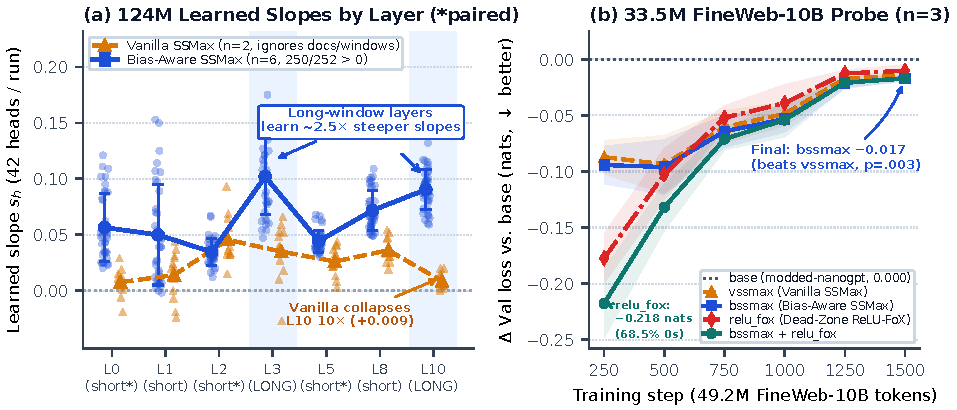
\includegraphics[width=\textwidth]{fig4_llm_mech.pdf}
  \caption{\textbf{Opening the 124M LLM black box + 33.5M FineWeb curves.}
  \textbf{(a)}~Real learned per-head slopes $s_{\ell,h}$ across all $7$ attention layers of $124\text{M}$ \texttt{modded-nanogpt} ($n=6$ centered low-LR runs = $252$ heads vs.\ $n=2$ Vanilla SSMax runs). Under Bias-Aware SSMax, $250/252$ heads ($99.2\%$) learn strictly positive slopes, and the two long-window layers (\texttt{L3}: $+0.102$, \texttt{L10}: $+0.090$, shaded) automatically learn $\sim 2.5\times$ steeper curves than short-window layers ($+0.035\text{--}0.072$). Under bias-blind Vanilla SSMax, \texttt{L10} collapses $10\times$ to $+0.009$.
  \textbf{(b)}~$33.5\text{M}$ FineWeb-10B validation loss delta vs.\ baseline ($n=3$): \texttt{relu\_fox} drops early loss by $-0.218$ nats (with $68.5\%$ exact-zero tokens), while \texttt{bssmax} wins cleanly at convergence.}
  \label{fig:llm_mech}
\end{figure}

\subsection{Mechanistic Interpretability Inside the 124M LLM}

What do those $42$ learned scalars actually do inside a $124\text{M}$ language model? Figure~\ref{fig:llm_mech}a plots every single learned head slope across all $7$ attention layers from our matched-step $G=52$ runs:
\begin{itemize}
  \item \textbf{Universal sharpening with visible length:} Across $6$ independent low-LR runs ($252$ heads total), \textbf{$250/252$ ($99.2\%$) heads} spontaneously learn strictly positive slopes $s_{\ell,h} > 0$.
  \item \textbf{Window-aware specialization:} In \texttt{modded-nanogpt}, layers \texttt{L0, L1, L2, L5, L8} use short sliding windows (reaching $640\text{--}768$ tokens), while \texttt{L3} and \texttt{L10} use long sliding windows (reaching $1{,}408\text{--}2{,}560$ tokens). Without being told which layers are long, Bias-Aware SSMax learns $\sim 2.5\times$ larger slopes on the two long-window layers (\texttt{L3}: $+0.102$, \texttt{L10}: $+0.090$) than on the short-window layers (\texttt{L2}: $+0.035$, \texttt{L5}: $+0.044$).
  \item \textbf{Why Vanilla SSMax breaks:} When given raw batch position instead of $\nvis$, the optimizer cannot trust the slope at document boundaries---so it crushes \texttt{L10}'s slope $10\times$ down to $+0.009$ and ends up \emph{worse} than unmodified \texttt{HEAD} ($3.2786$ vs.\ $3.2761$).
\end{itemize}

\subsection{Official \texorpdfstring{8$\times$H100}{8xH100} SXM5 Certification \& Variance Collapse}

\begin{figure}[t]
  \centering
  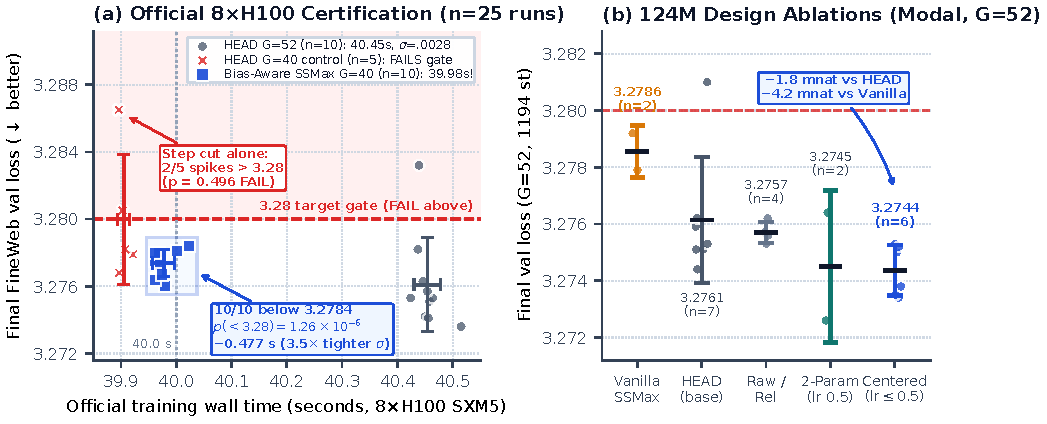
\includegraphics[width=\textwidth]{fig5_speedrun_cert.pdf}
  \caption{\textbf{Flagship $124\text{M}$ \texttt{modded-nanogpt} certification ($8\times\text{H100 SXM5}$) and matched-step ablations.}
  \textbf{(a)}~All $25$ official bare-metal Nebius runs plotted as wall-clock time vs.\ final validation loss against the $3.28$ gate (red dashed line). Cutting $12$ Stage-2 steps alone (\texttt{HEAD G=40}, red $\times$) fails the gate ($3.2800$, $2/5$ spikes, $p=0.496$). Adding centered Bias-Aware SSMax at the exact same $1{,}182$ steps (blue squares) hits \textbf{sub-40s ($39.977\text{ s}$, $-0.477\text{ s}$ vs.\ interleaved \texttt{HEAD})} with $10/10$ runs tightly clustered below $3.2784$ ($p=1.26\times 10^{-6}$, $3.5\times$ tighter $\sigma$).
  \textbf{(b)}~Matched-step ($G=52$, $1{,}194$ st) Modal design ablations ($n=27$ runs): centered $1$-parameter Bias-Aware SSMax beats both \texttt{HEAD} ($-1.8\text{ mnat}$) and Vanilla SSMax ($-4.2\text{ mnat}$) while cutting variance $>2.5\times$.}
  \label{fig:cert}
\end{figure}

Before touching the step schedule, we ran $27$ matched-step ($G=52$, $1{,}194$ steps) ablations on Modal $8\times\text{H100/H200}$ (Figure~\ref{fig:cert}b). Centered $1$-parameter Bias-Aware SSMax at $\text{lr\_mul} = 0.5$ achieved $3.27430 \pm 0.00099$ ($n=4$; pooled low-LR $\text{lr\_mul}\in\{0.25,0.5\}$, $n=6$: $3.27437 \pm 0.00089$), beating interleaved \texttt{HEAD} ($3.27614 \pm 0.00222$, $n=7$) by $-1.77\text{ mnat}$ (one-sided Welch $p=0.044$, two-sided $p=0.088$, Mann--Whitney $U$ $p=0.031$) and beating Vanilla SSMax ($3.27855 \pm 0.00092$, $n=2$) by $-4.25\text{ mnat}$ (two-sided $p=0.027$). Adding a second per-head intercept parameter (\texttt{2-Param}, $+84$ scalars) gave the same mean ($3.2745$) with $2.7\times$ worse variance, confirming that the simpler $1$-parameter centered form is strictly better.

We then ran the full certification on a bare-metal Nebius \texttt{8x NVIDIA H100 80GB HBM3} (\texttt{NV18} NVSwitch, \texttt{torch 2.10.0+cu128}, zero extra compiler flags, unmodified \texttt{run.sh}). Converting the $-1.8\text{ mnat}$ ML headroom into speed by trimming $12$ Stage-2 batch-$24$ steps (\texttt{SCHEDULE\_GROWTH\_STEPS: 52 $\to$ 40}, preserving exact mod-$4$ n-gram and mod-$2$ Adam boundary parity) yields the certification results in Table~\ref{tab:cert} and Figure~\ref{fig:cert}a:

\begin{table}[t]
  \centering
  \caption{$124\text{M}$ \texttt{modded-nanogpt} certification on bare-metal Nebius $8\times\text{H100 SXM5}$ ($10\text{ vs.\ }10$ interleaved A/B + $5$-run matched-step control) and Modal matched-step ($G=52$) ablations.}
  \label{tab:cert}
  \footnotesize
  \renewcommand{\arraystretch}{1.14}
  \setlength{\tabcolsep}{3.6pt}
  \begin{tabular}{@{}lrrcccrc@{}}
    \toprule
    Arm & $n$ & Steps & Wall Time & Final \texttt{val\_loss} & Range & $>3.28$ & $p(<3.28)$ \\
    \midrule
    \multicolumn{8}{@{}l}{\textit{\textbf{Bare-Metal Nebius $8\times\text{H100 SXM5}$ (Official Interleaved Certification + Matched-Step Control)}}} \\
    \texttt{HEAD} (\texttt{4ea6b93}, $G=52$) & 10 & 1194 & $40.454 \pm 0.024\text{ s}$ & $3.27610 \pm 0.00281$ & $3.2736\text{--}3.2832$ & $1/10$ & $8.78\times 10^{-4}$ \\
    \textbf{Bias-Aware SSMax ($G=40$)} & \textbf{10} & \textbf{1182} & \textbf{39.977 $\pm$ 0.020 s} & \textbf{3.27738 $\pm$ 0.00079} & \textbf{3.2760--3.2784} & \textbf{0/10} & \textbf{1.26$\times$10$^{-6}$} \\
    \texttt{HEAD @ G=40} (step-cut only) & 5 & 1182 & $39.905 \pm 0.011\text{ s}$ & $3.27998 \pm 0.00389$ & $3.2768\text{--}3.2865$ & $2/5$ & $0.496$ (\textbf{FAIL}) \\
    \midrule
    \multicolumn{8}{@{}l}{\textit{\textbf{Modal $8\times\text{H100/H200}$ (Matched-Step $G=52$ Design Ablations)}}} \\
    \texttt{HEAD} (base controls) & 7 & 1194 & --- & $3.27614 \pm 0.00222$ & $3.2744\text{--}3.2810$ & $1/7$ & --- \\
    Vanilla SSMax (\texttt{vssmax}) & 2 & 1194 & --- & $3.27855 \pm 0.00092$ & $3.2779\text{--}3.2792$ & $0/2$ & --- \\
    \textbf{Centered Bias-SSMax ($\text{lr}\le 0.5$)} & \textbf{6} & \textbf{1194} & --- & \textbf{3.27437 $\pm$ 0.00089} & \textbf{3.2734--3.2753} & \textbf{0/6} & --- \\
    \bottomrule
  \end{tabular}
\end{table}

\begin{itemize}
  \item \textbf{Sub-40s speedrun win:} Across $10$ adjacent interleaved pairs, Bias-Aware SSMax runs in $\mathbf{39.977 \pm 0.020\text{ s}}$ vs.\ \texttt{HEAD}'s $40.454 \pm 0.024\text{ s}$---\textbf{$-0.477 \pm 0.034\text{ s}$ ($-1.18\%$)}, two-sided paired $p = 7.62\times 10^{-12}$---while clearing the $3.28$ gate at $3.27738 \pm 0.00079$ ($t = -10.43$, one-sided $p = 1.26\times 10^{-6}$).
  \item \textbf{Not just a step cut:} Cutting the exact same $12$ steps from \texttt{HEAD} without SSMax (\texttt{HEAD @ G=40}, $n=5$) degrades loss to $3.27998 \pm 0.00389$ ($2/5$ runs above $3.28$: $3.2805, 3.2865$, $p=0.496$---fails the gate!). At identical step count, Bias-Aware SSMax is \textbf{$-2.60\text{ mnat}$ better} with \textbf{$4.9\times$ tighter variance} for only $+72\text{ ms}$ kernel cost (an estimated $\sim 354\text{ ms}$ net matched-loss speedup, and an implied $373\text{ ms/mnat}$ slope vs.\ ANVIL2's $164\text{ ms/mnat}$ step-cut slope).
  \item \textbf{Why run-to-run variance collapses across both clouds:} Across all $22$ unmodified \texttt{HEAD} runs on Modal and Nebius combined, \texttt{HEAD} spiked above $3.28$ four times ($3.2810, 3.2832, 3.2805, 3.2865$). Across all $16$ centered low-LR Bias-Aware SSMax runs on both clouds, \textbf{zero runs exceeded $3.2784$} ($3.5\text{--}4.9\times$ tighter std). Packed batches randomly mix short and long documents; fixed temperature leaves long-window queries under-sharpened and fresh document starts over-sharpened. Adapting $\tau$ to each token's exact visible context stabilizes attention entropy across random batches and random seeds.
\end{itemize}

% =============================================================================
\section{When to Use What \& Honest Limitations}
\label{sec:disc}

Taken together, our experiments across four benchmarks ($112\text{k}$ to $124\text{M}$ parameters) reveal a clean practical rule of thumb:

\begin{itemize}
  \item \textbf{Use Bias-Aware SSMax everywhere.} In its closed-form window/document version (Eq.~\ref{eq:nvis}), it costs $+1$ scalar per head, $+0\text{ MiB}$ VRAM, and $+0.17\%$ runtime when fused into QK-RMSNorm+RoPE, yet improves accuracy, length extrapolation, and run-to-run stability across arithmetic, symbolic algebra, $33.5\text{M}$ FineWeb, and the $124\text{M}$ $8\times\text{H100}$ speedrun---beating bias-blind Vanilla SSMax on every single task.
  \item \textbf{Add Barrier-FoX / Dead-Zone $\operatorname{ReLU}$-FoX when exact long-range state resets cannot be approximated by a fixed window.} On carry chains ($+59\text{pp}$ at $5\times$, $71.9\%$ on $40$-digit pure-$9$ chains) and multi-step symbolic rewriting ($+10.4\text{pp}$ convergence), learned walls are transformative. On short-window prose pretraining where hard sliding windows and \texttt{<|endoftext|>} masks already perform most resets, \texttt{relu\_fox} dramatically speeds up early training ($-0.218$ nats at step $250$) while self-discovering $68.5\%$ exact-zero tokens, but converges to parity with Bias-Aware SSMax alone.
\end{itemize}

\textbf{Limitations.}
(1)~Hard $\operatorname{ReLU}$ barrier gates eliminate carry leakage completely on pure-$9$ chains ($71.9\%$) at the cost of higher dead-gate variance across random seeds on general sums; smoother dead-zone schedules (e.g., annealing from $\operatorname{softplus}$ to $\operatorname{ReLU}$) remain open.
(2)~Place-Ordered Barrier-FoX uses digit place IDs specific to positional notation, whereas Token-FoX and Bias-Aware SSMax are completely domain-agnostic.
(3)~We tested Bias-Aware SSMax up to $124\text{M}$ parameters / $3\text{k}$ context and \texttt{relu\_fox} under short sliding windows; validating both on full-context ($8\text{k--}32\text{k}$) billion-parameter models without short windows is a natural next step.

\vspace{6pt}
\begingroup
\small
\setlength{\itemsep}{2.5pt}\setlength{\parskip}{0pt}
\begin{thebibliography}{11}
\bibitem{chiang2022} D.~Chiang and P.~Cholak. Overcoming a theoretical limitation of self-attention. \emph{ACL}, 2022.
\bibitem{jordan2024} K.~Jordan et~al. \texttt{modded-nanogpt} and Muon: An optimizer for hidden layers in neural networks, 2024. \url{https://github.com/KellerJordan/modded-nanogpt}.
\bibitem{kazemnejad2023} A.~Kazemnejad, I.~Padhi, K.~N. Ramamurthy, P.~Das, and S.~Reddy. The impact of positional encoding on length generalization in transformers. \emph{NeurIPS}, 2023.
\bibitem{lin2025} Z.~Lin, E.~Nikishin, X.~He, and A.~Courville. Forgetting Transformer: Softmax attention with a forget gate. \emph{ICLR}, 2025.
\bibitem{mcleish2024} S.~McLeish et~al. Transformers can do arithmetic with the right embeddings. \emph{NeurIPS}, 2024.
\bibitem{nakanishi2025} K.~M. Nakanishi. Scalable-Softmax is superior for attention. \emph{arXiv:2501.19399}, 2025.
\bibitem{penedo2024} G.~Penedo et~al. The FineWeb datasets: Decanting the web for the finest text data at scale. \emph{NeurIPS Datasets \& Benchmarks}, 2024.
\bibitem{press2022} O.~Press, N.~A. Smith, and M.~Lewis. Train short, test long: Attention with linear biases enables input length extrapolation. \emph{ICLR}, 2022.
\bibitem{shazeer2020} N.~Shazeer. GLU variants improve Transformer. \emph{arXiv:2002.05202}, 2020.
\bibitem{su2024} J.~Su, M.~Ahmed, Y.~Lu, S.~Pan, W.~Bo, and Y.~Liu. RoFormer: Enhanced transformer with rotary position embedding. \emph{Neurocomputing}, 568:127063, 2024.
\bibitem{velickovic2025} P.~Veli{\v{c}}kovi{\'c}, C.~Perivolaropoulos, F.~Barbero, and R.~Pascanu. Softmax is not enough (for sharp size generalisation). \emph{arXiv:2410.01104} (ICML 2025), 2024.
\end{thebibliography}
\endgroup

\end{document}
